% !TEX root = Stolpe_2018_Thesis.tex
% !TEX encoding = UTF-8

\chapter{Experience Report}
\label{cha:evaluation}

In \autoref{cha:implementation}, we have shown how \graallsp~was implemented. To support all the described \ac{lsp} features, language implementations need to implement existing Truffle \acp{api} and our proposed extensions. For some languages, this might be done with very low implementation effort, but for others, some features might require fundamental changes in their implementations. In this chapter, we show by means of the dynamic Truffle languages GraalPython, SimpleLanguage, FastR, and GraalSqueak, that a basic support of some \ac{lsp} features can be achieved with minimal implementation effort. Furthermore, we explain, why certain \ac{lsp} features cannot be easily supported in some language implementations. Finally, we describe limitations of our approach and implementation of \graallsp. 

\section{Comparison of Truffle Language Implementations}
\label{sec:xp:ComparisonOfLangImpls}

\acf{sl}\footnote{\url{https://github.com/graalvm/simplelanguage} (accessed 2018-12-17)} is Truffle's exemplary language implementation, to showcase Truffle features and help understanding its ideas and concepts. \ac{sl} has first class functions. The type system only consists of primitive types and a single \inlinecode{object} type. Objects are implemented as simple key-value stores. As showcase implementation, it implements most of the needed Truffle \acp{api} so that, after implementing our proposed extensions with minimal effort, \ac{sl} supports nearly all \graallsp~features.

GraalPython\footnote{\url{https://github.com/graalvm/graalpython} (accessed 2018-12-17)} is an early-stage experimental implementation of Python. It does not support many libraries yet, but is mature enough for our use cases. Together with the GraalPython team, we implemented the required Truffle \acp{api}, so that GraalPython is the language implementation which supports the most \graallsp~features now.

FastR\footnote{\url{https://github.com/oracle/fastr} (accessed 2018-12-17)} is a high-performance implementation of the R\footnote{\url{https://www.r-project.org} (accessed 2018-12-17)} programming language used for statistical computing and graphics. Its goal is to become a drop-in replacement for the reference implementation GNU-R. Due to time constraints, we have only implemented support for completion trigger characters yet, so that the FastR implementation is nearly unchanged. Therefore, not many \graallsp~features are supported.

GraalSqueak\footnote{\url{https://github.com/hpi-swa-lab/graalsqueak} (accessed 2018-12-17)} \cite{niephaus2018graalsqueak} is an early-stage experimental Squeak/Smalltalk \cite{ingalls1997back} implementation. In contrast to the other selected languages, it is an image-based, graphical live-programming environment. Furthermore, it uses the \ac{ast}-based Truffle framework to implement a bytecode interpreter. Therefore, it is difficult to map concepts of GraalSqueak to the file-based \ac{lsp} protocol. Nonetheless, we have chosen it to show that at least some features can be supported with reasonable effort and to discuss limitations of our approach. We run GraalSqueak in headless mode to load an image and get access to its run-time objects. For now, we treat every opened \inlinecode{*.st} file as an isolated Squeak/Smalltalk workspace.

%For SL, the implemented extensions are already available as public GitHub pull requests. For GraalPython, FastR, and GraalSqueak, we implemented ... \todo{}

\autoref{tab:truffleAPIXLanguageMatrix} gives an overview over the status quo of implemented Truffle \acp{api} of these languages. Futhermore, \autoref{tab:lspFeatureXLanguageMatrix} adds a broad overview over the resulting \graallsp~features supported by these languages. In the following, we will highlight, how well some of these features are already supported by showing and describing screenshots of the usage in a language client. Therefore, we have built a small extension in Visual Studio Code, which connects to an already running \graallsp~instance.

\newcommand{\cmark}{\ding{51}}
\newcommand{\xmark}{\ding{55}}
\newcommand{\nyi}{\xmark}


\begin{table}
    \centering
    \tableinsidecommand
    \begin{threeparttable}
      \caption[Language overview of supported Truffle \acp{api}]{An overview over selected Truffle languages and their current support of existing Truffle \acp{api} and our proposed extensions. Adjusting and extending these language implementations for \graallsp~is still work in progress, especially for FastR and GraalSqueak.}
      \label{tab:truffleAPIXLanguageMatrix}
      \begin{tabular}{ l c c c c }
        \toprule
        Truffle \ac{api} (existing and extensions)     & SL & GraalPython & FastR & GraalSqueak \\
        \midrule
        CallTag                                         & \cmark & \cmark & \cmark & \xmark \\
        StatementTag                                    & \cmark & \cmark & \cmark & \cmark \\
        ExpressionTag                                   & \cmark & \cmark & \nyi & \nyi \\
        findTopScopes()                                 & \cmark & \cmark & \cmark & \cmark \\
        findLocalScopes()                               & \cmark & \cmark & \cmark\tnote{r} & \nyi \\
        findMetaObject()                                & \cmark\tnote{n} & \cmark & \cmark\tnote{n} & \cmark \\
        findSourceLocation()                            & \cmark & \cmark & \cmark & \nyi\tnote{?} \\
        parse() eager \ac{ast} creation                 & \cmark & \cmark & \cmark & \xmark \\
        parseInline()                                   & \xmark & \cmark & \cmark & \nyi \\
        \midrule
        getCompletionTriggerCharacters()                & \cmark & \cmark & \cmark & \cmark \\
        getSignatureHelpTriggerCharacters()             & \nyi & \cmark & \nyi & \nyi \\
        getNodeObject() for literal nodes               & \cmark & \cmark & \nyi & \nyi \\
        boxPrimitive()                                  & \xmark & \cmark & \nyi & \nyi \\
        GetSignature custom message                     & \xmark & \cmark & \nyi & \nyi \\
        GetDocumentation custom message                 & \xmark & \cmark & \nyi & \nyi \\
        DeclarationTag, Read/WriteVariableTag           & \cmark & \cmark & \nyi & \nyi \\
        \bottomrule
      \end{tabular}
      \begin{tablenotes}
        \item [r] Run-time scopes only
        \item [n] Names of meta-objects only
        \item [?] Unclear how to implement
      \end{tablenotes}
    \end{threeparttable}
\end{table}


\begin{table}
    \centering
    \tableinsidecommand
    \begin{threeparttable}
      \caption[Language overview of supported \graallsp~features]{An overview over selected Truffle languages and their support of \graallsp~features. If a feature is not supported, it will either depend on not yet implemented Truffle \acp{api} as described in \autoref{tab:truffleAPIXLanguageMatrix}, or on missing information due to a run-time focused language implementation.}
      \label{tab:lspFeatureXLanguageMatrix}
      \begin{tabular}{ l c c c c }
        \toprule
        \ac{lsp} feature        & SL & GraalPython & FastR & GraalSqueak \\
        \midrule
        Diagnostics             & \cmark & \cmark & \xmark & \cmark \\
        Completion (globals)    & \cmark & \cmark & \cmark & \cmark \\
        Completion (locals)     & \cmark & \cmark & \cmark\tnote{*} & \xmark \\
        Completion (properties) & \cmark\tnote{*} & \cmark\tnote{*} & \xmark & \xmark \\
        Signature Help          & \xmark & \cmark\tnote{*} & \xmark & \xmark \\
        Hover                   & \cmark\tnote{*} & \cmark\tnote{*} & (\cmark)\tnote{*} & \xmark \\
        Symbols                 & \cmark & \cmark & (\cmark) & \xmark \\
        Goto-definition (callables)              & \cmark\tnote{*} & \cmark\tnote{*} & \cmark\tnote{*} & \xmark\tnote{?}  \\
        Goto-definition (local variables)              & \cmark & \cmark & \xmark & \xmark \\
        References (static)     & \cmark & \cmark & \xmark & \xmark\tnote{?} \\
        Variable Highlighting   & \cmark & \cmark & \xmark & \xmark \\
        \bottomrule
      \end{tabular}
      \begin{tablenotes}
        \item [*] Requires run-time information
        \item [()] Larger limitations
        \item [?] Unclear how to implement
      \end{tablenotes}
    \end{threeparttable}
\end{table}

\paragraph{Diagnostics}
All languages except FastR fail parsing at the first syntax error, so that only one error per file can be sent to the client. \autoref{fig:xp:diagnosticsSL} displays how such a diagnostics notification is visualized in \ac{sl}. FastR does not throw a \inlinecode{TruffleException} in case of a syntax error, so that \graallsp~cannot report any syntax errors for FastR.
%GraalSqueak does not support eager parsing yet, so that we have to execute the code to trigger the actual parsing. Then, the first syntax error is reported via a \inlinecode{TruffleException}.

\begin{figure}
    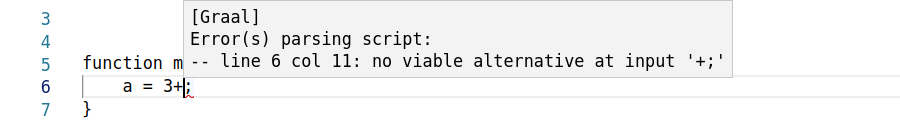
\includegraphics[width=\linewidth]{images/xp_report/diagnostics_sl.png}
    \caption[Diagnostics used to display a syntax error in \acs{sl}]{Diagnostics used to display a syntax error in \acs{sl}.}
    \label{fig:xp:diagnosticsSL}
\end{figure}

\paragraph{Code Completion}
\autoref{fig:xp:completionGlobalsPython} shows a code completion for globals and locals in GraalPython. Completion items have different icons for classes, methods, and variables in the list of suggestions. For the selected item of a built-in class, a string representation of the corresponding meta-object is displayed, together with a documentation, if available. \autoref{fig:xp:completionLocalsSL} shows a code completion in \ac{sl}. Variables of lexical local scopes are listed first, followed by built-in functions. For the selected local variable, the scope name is displayed. \autoref{fig:xp:completionGlobalsR} shows a completion of globals in FastR, with an already filtered list of globals containing the string \inlinecode{"as"}. The completion of locals in FastR is supported only if run-time information, i.e. a frame, is available. \autoref{fig:xp:completionGlobalsGraalSqueak} shows globals of the Smalltalk dictionary for GraalSqueak.

\begin{figure}
    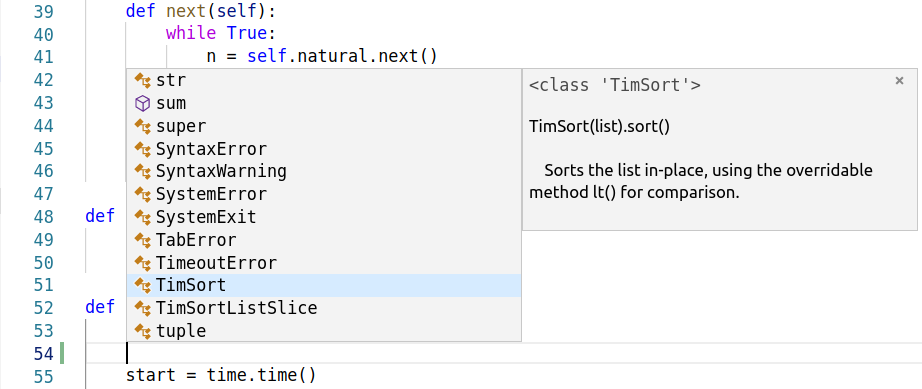
\includegraphics[width=\linewidth]{images/xp_report/code_completion_globals_python_with_docu.png}
    \caption[Code completion of globals and locals in GraalPython]{Code completion of globals and locals in GraalPython.}
    \label{fig:xp:completionGlobalsPython}
\end{figure}

\begin{figure}
    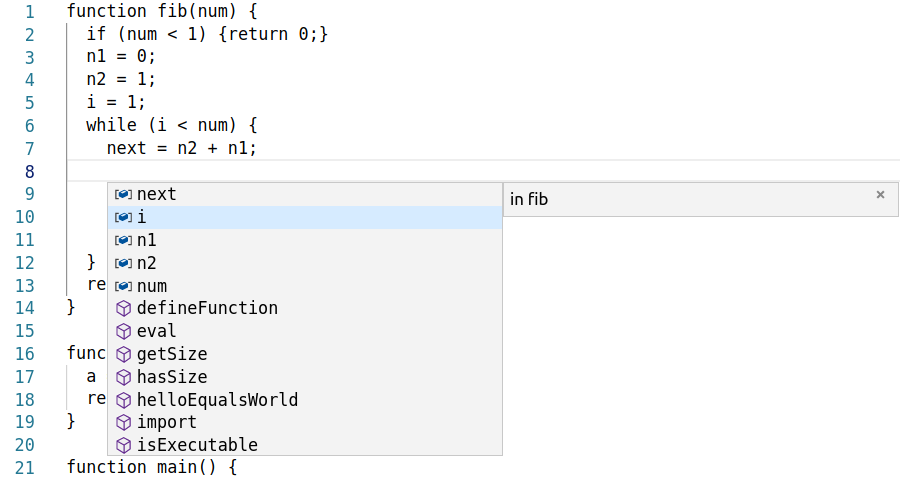
\includegraphics[width=\linewidth]{images/xp_report/code_completion_locals_sl.png}
    \caption[Code completion of globals and locals in \acs{sl}]{Code completion of globals and locals in \acs{sl}.}
    \label{fig:xp:completionLocalsSL}
\end{figure}

\begin{figure}
    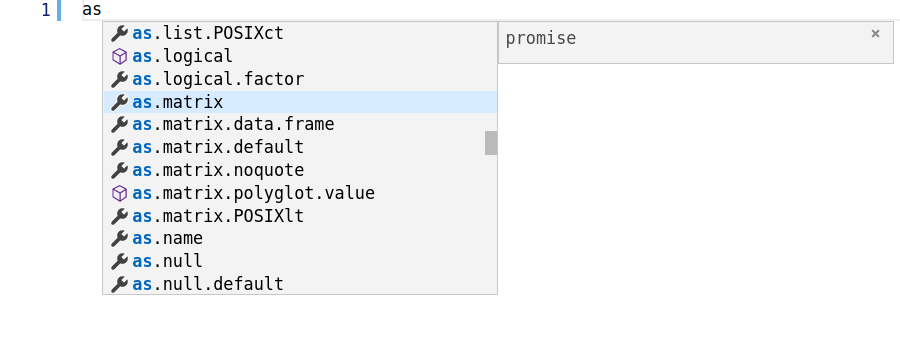
\includegraphics[width=\linewidth]{images/xp_report/code_completion_globals_R.png}
    \caption[Code completion of globals in FastR]{Code completion of globals in FastR.}
    \label{fig:xp:completionGlobalsR}
\end{figure}

\begin{figure}
    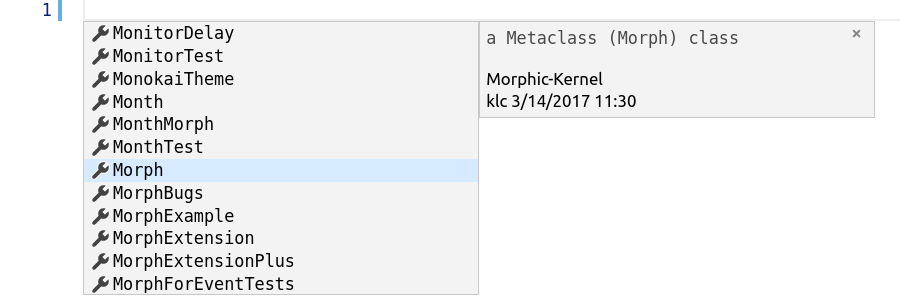
\includegraphics[width=\linewidth]{images/xp_report/code_completion_globals_GraalSqueak.png}
    \caption[Code completion of globals in GraalSqueak]{Code completion of globals in GraalSqueak.}
    \label{fig:xp:completionGlobalsGraalSqueak}
\end{figure}

The code completion of properties is supported to different extents in these languages. Run-time information are always required due to the dynamic nature of the languages. Therefore, the source code needs to be parsable after removing the trigger character. For \ac{sl}, \graallsp~supports the completion of properties, which are the keys of the underlying key-value store. For GraalPython, properties of objects can also be those inherited from their type hierarchy including fields and methods of their classes. For FastR and GraalSqueak, we were not able to provide a completion of properties yet, due to the missing support of \inlinecode{ExpressionTag} annotations for their \ac{ast} nodes. But also for languages supporting the \inlinecode{ExpressionTag}, the applicability of our approach depends on the design of their \ac{ast}. In GraalPython, triggering a completion in the code snippet \inlinecode{anObject.nestedObject} by inserting a dot at the end, will yield completion items for all properties of the object referenced by \inlinecode{anObject.nestedObject}, because the nearest node tagged with an \inlinecode{ExpressionTag} is the one representing the whole source section. In \ac{sl} however, inserting a dot before the semicolon in \inlinecode{anObject.nestedObject;} to trigger code completion, will yield no results, because the nearest node tagged with an \inlinecode{ExpressionTag} is the \inlinecode{SLStringLiteralNode} instance representing \inlinecode{nestedObject} and not the node representing \inlinecode{anObject.nestedObject}. Therefore, our approach tries to derive completion items from the String \inlinecode{"nestedObject"}, which is the execution result of the \inlinecode{SLStringLiteralNode} instance. Similar cases might occur also in other language implementations, because Truffle leaves the \ac{ast} design to the language implementors, so that \graallsp~can only be implemented as language-agnostic best-effort approach.

Using GraalPython and \ac{sl}, we want to highlight, that Truffle supports polyglot programming and we can therefore provide completion of properties across language boundaries. \autoref{fig:xp:completionPolyglot} shows Python code evaluating a \ac{sl} code snippet which creates and returns a \ac{sl} object. In the last line, we get completions of properties for the foreign \ac{sl} object, which would not be possible in \ac{sl} code, as described in the previous paragraph.

The code completion request for properties is triggered fairly often in comparison to the other run-time information requiring requests. Unfortunately, the performance depends on the one hand on the execution time of the source code, which can be reduced by caching run-time information, but on the other hand it depends on the creation time of Truffle language contexts. We create a new one for each execution, which is quite cheap for \ac{sl}, but for GraalPython, it takes a noticeable time. Reusing those contexts improves the performance, but introduces new problems, which we will explain in detail in \autoref{sec:xp:limitations}.

\begin{figure}
    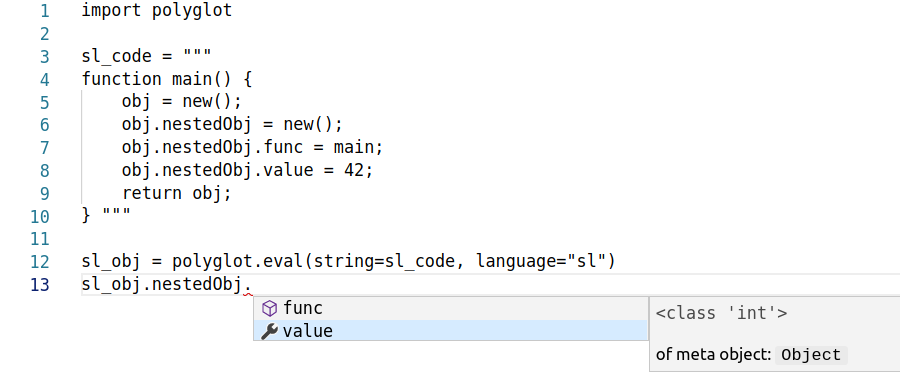
\includegraphics[width=\linewidth]{images/xp_report/completion_properties_polylgot.png}
    \caption[Polyglot code completion of properties]{Completion of properties for a foreign \acs{sl} object in GraalPython source code.}
    \label{fig:xp:completionPolyglot}
\end{figure}

\paragraph{Signature Help}
Signature help is only supported with limitations for GraalPython yet. \graallsp~can provide a formatted signature string as shown in \autoref{fig:xp:signatureHelpPython}, but when starting to fill in the signature, the displayed hint will be cancelled as soon as a syntax error is reported. For example when typing \inlinecode{"string="}, to define a keyword argument. Afterwards, the signature help request is not triggered again. The other languages do not support the \inlinecode{GetSignature} custom message yet. Implementing this message for example in \ac{sl} might not be possible without changes to the language, because \ac{sl} stores function arguments internally like any other local variable of the function, so that there is no knowledge left at run-time to obtain the signature of a function. This is one example of many, where languages need to store additional parse-time information, to support more \ac{lsp} features.

\begin{figure}
    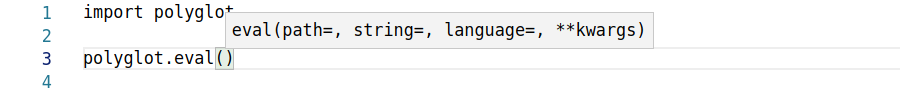
\includegraphics[width=\linewidth]{images/xp_report/signature_help_python.png}
    \caption[Signature help for GraalPython]{Signature help for GraalPython.}
    \label{fig:xp:signatureHelpPython}
\end{figure}

\paragraph{Hover}
Showing information on mouse hover is supported for variables and expressions of \ac{sl} and GraalPython yet. For FastR, only variables can be accessed via their corresponding frame slot, to provide hover information. For all languages, cached run-time information need to be available. A collection run can be triggered using the \emph{codeLense} named \inlinecode{"Analyse coverage"}, as shown above the first line of code in \autoref{fig:xp:hoverR}. The displayed hover information include a string representation of the variable's value and the meta-object.


\begin{figure}
    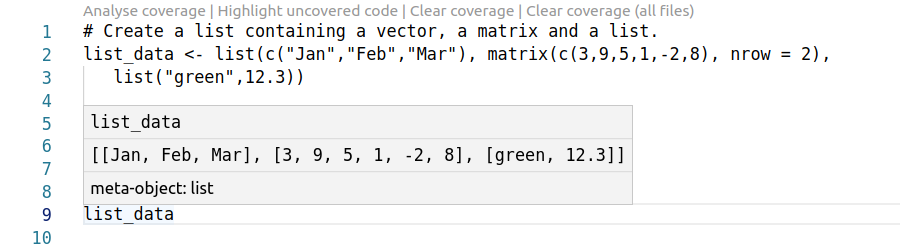
\includegraphics[width=\linewidth]{images/xp_report/hover_R.png}
    \caption[Hover information in FastR source code]{Displaying information on mouse hover for FastR source code using cached run-time information.}
    \label{fig:xp:hoverR}
\end{figure}

\paragraph{Symbols}
As soon as a language eagerly creates \ac{ast} nodes when the source code is parsed, \graallsp~can support the request for symbols by providing the names of all \inlinecode{RootNode} instances in the current document. If the \inlinecode{DeclarationTag} is used to annotate nodes, we can access further information to set a fitting symbol type and container name as shown for GraalPython in \autoref{fig:xp:symbolsPython}. For FastR however, taking the names of all \inlinecode{RootNode} instances is not useful yet, because there is one for each line with the name \inlinecode{<repl wrapper>}.

\begin{figure}
    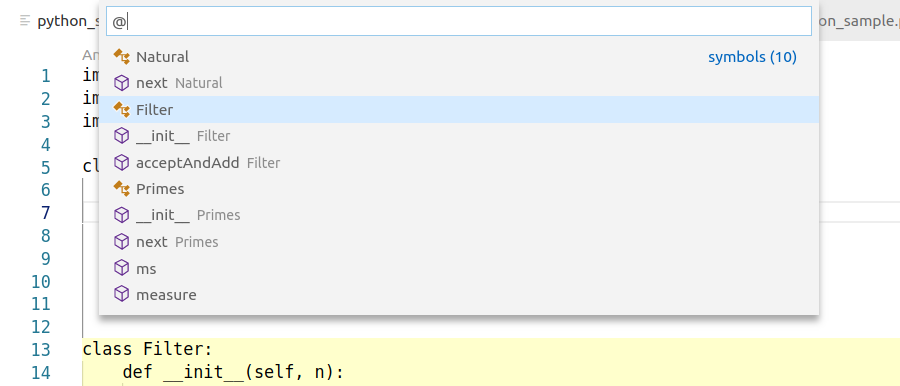
\includegraphics[width=\linewidth]{images/xp_report/symbols_Python.png}
    \caption[Symbol overview in GraalPython]{Symbol overview over the current GraalPython document. The selected entry's source section is highlighted in the editor.}
    \label{fig:xp:symbolsPython}
\end{figure}

\paragraph{Goto-definition and References}
%Our Goto-definition implementation for callables might behave a bit unexpected for languages having first class functions like GraalPython or \ac{sl}. It is not always obvious, if a goto-definition request targets the variable which is read to get the callable object, or the callable itself. For example, for GraalPython  \inlinecode{} . Additionally, the behavior of our implementation depends on the language support. If \inlinecode{ReadVariableTag} and \inlinecode{WriteVariableTag} are supported, we can differentiate between a jump to the variable definition and a jump to the callable definition. Otherwise we will always jump to the callable definition.
Our goto-definition and find-all-references implementations depend on the supported tags of the Truffle language. The selected languages, except GraalSqueak, use the \inlinecode{CallTag} to annotate nodes representing a call, so that goto-definition can be supported using run-time information. This works also across language boundaries, when using Truffle's polyglot \ac{api}. Find-all-references uses a static symbol search yet, so that it will work as soon as the code is parsable. To avoid too much false-positive matches, we disabled the search in internal sources of the language by default. For GraalSqueak, which is not file-based, we do not know yet, how a useful implementation of navigational requests might look like in general.

\paragraph{Variable Highlighting}
The support for highlighting of variable accesses depends on the usage of \inlinecode{ReadVariableTag} and \inlinecode{WriteVariableTag}. \autoref{fig:xp:highlightingPython} shows how it looks like for GraalPython. As for \ac{sl}, the node's source section, representing a variable write access, does not only cover the variable name, but also the right-hand side of the assignment. This might be fine for the highlighting use case, but it makes it more difficult to implement for example the \ac{lsp} \emph{rename} request for local variables, because we would have to locate the variable's identifier in the source section by ourselves.

\begin{figure}
    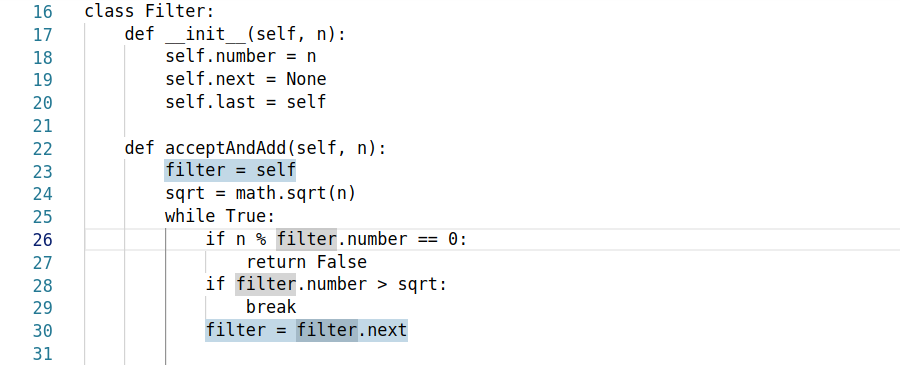
\includegraphics[width=\linewidth]{images/xp_report/highlighting_Python.png}
    \caption[Highlighting of variable accesses in GraalPython]{Highlighting of variable accesses in GraalPython. The source sections of write accesses cover the whole assignment and are highlighted in a blueish shade.}
    \label{fig:xp:highlightingPython}
\end{figure}




% \paragraph{GraalPython, SL, (Graal.js), FastR usage check}
% \begin{itemize}
%     \item matrix of \graallsp~features x Truffle languages
%     \item list SLOC for adjustments of these langs
%     \item matrix of \graallsp~features x Truffle languages without language adjustments? Should be only completion of globals/locals and static stuff possible -> or add a footnote in the first matrix, to mark that it is only working with adjustments
%     \item include screenshots of VSCode for important LSP features, put rest in appendix?
% \end{itemize}

% \paragraph{other stuff}
% \begin{itemize}
%     \item Completion response time
%     \item Eat your own dog food - Hover: We used the static hover information ourselves during implementation.
%     \item Between IDE and Language Workbench
% \end{itemize}
    

% \paragraph{Between IDE and Language Workbench}
%     Language Workbench focus/aim: Efficient language (DSL) development, performance is not main focus
%     vs. Graal/Truffle aim: Efficient execution

%     Assumption: Language Workbenches use static information only, our Truffle-based solution uses dynamic type information

\section{Limitations of \graallsp}
\label{sec:xp:limitations}
\begin{itemize}
    %\item Server: Only TCP (connecting to already running server), no std-in/-out impl + typically a language server life cycle is controlled by the client (start+shutdown). Our impl started external.
    %\item Truffle: Only first syntax error is reported. Lang parsers fail on first error
    %\item Cancellation of requests not yet supported
    %\item also, this in-line eval is interpretation only
    %\item sandboxing limited to fie I/O + read-only FS atm
    %\item limitations due to caching of last nested context - show example of dirty context, e.g. function renamed
    %\item Using cached run-time infos: we have frame but to do in-line eval we call node.execute(frame) ourselves without having a valid execution stack there -> if the execution relies on the stack, it will not work
    %\item Context creation time expensive
    %\item performance
    \item \todo{open limitations}type harvesting: we take a snapshot of the frame for the first entering of a source section -> different types for a frame slot are ignored
    \item memory consumption? We avoid GC of lots of objects by caching frames.
    %\item the snapshot taken copies frame and descriptor, but no deep copy of objects is done. Therefore the reference to these objects will represent the last state of execution

    %\item Graal compiler optimizations -> overhead for short scripts?!
    %\item typically one lang per server -> dynamic detection of languages + polyglot makes impl harder
    %\item example: Using R and Python -> R has dot in names of globals, for Python it is a trigger char -> dot char interrupts current completion, because a new one is triggered \autoref{fig:xp:completionGlobalsR}
    
    \item TruffleObject KEYS not hierarchical
    %\item code completion of properties only possible if dot is the last char inserted
\end{itemize}
Due to time constraints and limitations of the Truffle framework, we were unable to fully implement the approach described in \autoref{cha:solution}. We have not yet implemented a timeout or cancellation support for requests, to avoid an endless execution of source code when collecting run-time information. The suggested sandboxing of the execution engine is limited to file I/O for now, because Truffle does not support restriction of other I/O kinds yet. Furthermore, the sandbox is always activated when source code is executed, because we have not yet implemented a possibility to deactivate sandboxing when the user classifies the occurring side-effects as uncritical. Therefore, all features of \graallsp, which require collecting run-time information, are not be supported yet, if the executed source code requires write access to the file system. For GraalSqueak, this is a serious limitation, because it continuously stores actions and source code modifications of the current image in a separate \inlinecode{*.changes} file and wants therefore to open this file with write permissions during start-up. This fails at the moment due to our read-only file system, so that the whole image is not initialized correctly and we are unable to retrieve documentations for classes for example yet. 

\paragraph{Limitations of Caching Run-time Information and Reusing Contexts}
As described in \autoref{sec:impl:obtainingRunTimeInfos}, we introduced caching of run-time information and reusing of Truffle language contexts, to improve performance especially for code completion. Unfortunately, this implies some new limitations. To cache run-time information, we create a snapshot of the current \inlinecode{MaterializedFrame} instance at a specific source section. This snapshot is not a deep frame copy, so that only primitive values are actually copied. If fields of referenced objects are changed later, the frame snapshot will still reference these mutated objects. \autoref{fig:xp:limitationCachedCompletionPython} illustrates the problem using a GraalPython code snippet.

\begin{figure}
    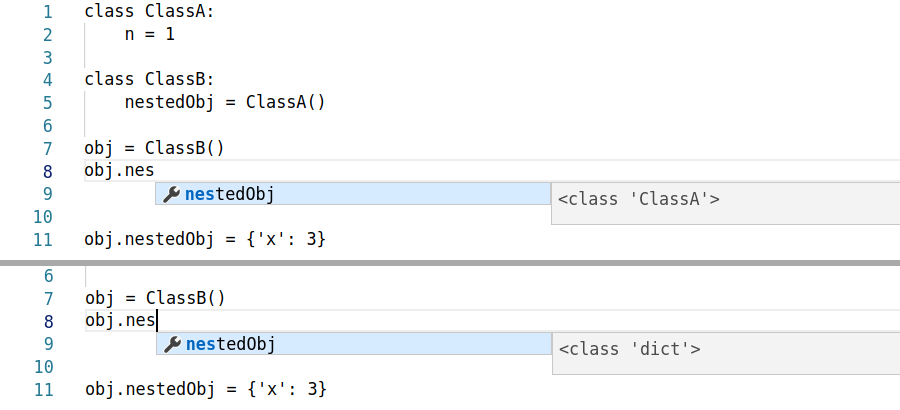
\includegraphics[width=\linewidth]{images/xp_report/limitation_cached_completion_Python.png}
    \caption[Limitations of code completion using cached run-time information]{Code completion of properties without and with cached run-time information in GraalPython. In the upper part of the image, the completion is shown as expected, because the completion items were obtained from the run-time state at line 8 by executing the source code up to that line. In the lower part, run-time information have been collected for the whole source code and the completion items were obtained from the frame snapshot stored in line 7, whose stored \inlinecode{obj} instance is no deep copy and therefore includes the modification in line 11.}
    \label{fig:xp:limitationCachedCompletionPython}
\end{figure}

Using cached frames for in-line evaluation, to improve the performance of \ac{lsp} responses, has another limitation. The executed source code must only rely on data of the stored frame snapshot. There is for example no call stack available and the language context storing the global run-time state might be different than it was at the moment when the snapshot was taken.

As already mentioned, we also reuse language contexts to avoid their expensive creation each time source code has to be executed. Unfortunately, this leads to similar global state problems as described for stored frame snapshots. For example in GraalPython, a module import is done only once per context. If the module's source code is changed and we reuse a context which has already imported that module, the changes will be ignored in further executing runs. Furthermore, after renaming functions, the old ones will still be suggested via code completion.

With regard to the numerous limitations which arise due to our current implementation of caching run-time information, we have to admit, that this part needs further improvements. It works well for context independent scripts, but is not yet mature enough for lager software projects.

\paragraph{Limitations of a Polyglot Language Server}
The Truffle framework allows to host language implementations in a multi-language run-time environment. We have already explained, that \graallsp~supports polyglot code completion, but this causes some limitations. A language server is typically developed for exactly one language. During initialization we have to tell the language client the set of completion and signature help trigger characters to support auto-activation. If the installed languages have different trigger characters, like a dot for GraalPython, a \inlinecode{\$} for FastR, and a space for GraalSqueak, a completion might be triggered in unwanted situations and might cancel other requests. FastR for example allows to use dots in variable identifiers, as can be seen in the already mentioned \autoref{fig:xp:completionGlobalsR}. Typing a dot in FastR code while having GraalPython installed, will trigger a code completion request. At server-side, we can detect, that the dot is no trigger character of FastR and return no completion items, but the current request, which might be a previous completion request of FastR, will be cancelled. Furthermore, Visual Studio Code displays a default, token-based code completion, if \graallsp~ returns no results. This is quite confusing for the language users, because a language's code completion behavior might change depending on the other installed languages.


\section{Limitations of Our Approach}
\begin{itemize}
    \item LSP: Syntax highlighting defined at client-side, semantic coloring is on the agenda of the \ac{lsp} specification team and might be supported in a future version of \ac{lsp}. It remains to be seen, if semantic coloring might be exploited to provide a complete syntax highlighting from server-side.
    \item LSP+VSCode: Need to define supported languages in extension up-front
    \item LSP: No incremental sending of (completion) results
    \item LSP: has file-based code focus (GraalSqueak integration really hard)
    \item Run-time type collection / type harvesting
        \begin{itemize}
            \item caching is poorly conceived: storing frames / objects -> memory? + in-line eval without call stack difficult
            \item framework needs to support instrumentation / tracing to find the desired run-time object
            \item needs possibility to query the resulting host language object about its guest language semantics (e.g. a TruffleObject understanding a KEYS message)
            \item we query the actual run-time object, which might be really specialized, whereas type harvesting builds generalizations on seen types and yields only the generalized type
        \end{itemize}
    \item Reusing run-time focused parser: Only first syntax error is reported. Lang parsers fail on first error.
    \item We will not be able to compete with a language-specific language server
    \item Out of the box support for every language client is not given -> still need to implement an extension / lsp adapter at client-side
\end{itemize}


%%% Local Variables:
%%% mode: latex
%%% TeX-master: "Stolpe_2018_Thesis"
%%% coding: utf-8
%%% End:
